% vim:encoding=utf8 ft=tex sts=2 sw=2 et:
% Copyright (c) 2009 Jaroslaw Koszuk
%
% $Id$

\documentclass{tewiart}

\usepackage[utf8]{inputenc}
\usepackage[T1]{fontenc}
\usepackage{graphicx}
\usepackage{amsthm}
\usepackage{txfonts}
\usepackage{epstopdf}
\usepackage{placeins}
\usepackage[english]{babel}
\usepackage[utf8]{inputenc}
\usepackage[table]{xcolor}
\usepackage{array}
\usepackage{subcaption}

\newtheorem{definition}{Definition}
\newtheorem{theorem}[definition]{Theorem}
\newtheorem{corollary}[definition]{Corollary}
\newtheorem{proposition}[definition]{Proposition}
\newtheorem{example}[definition]{Example}


\title{Magnitude of simple rules in investment strategies of algorithmic trading}
\headtitle{Magnitude of simple rules in investment strategies of algorithmic trading\dots}
\author{Antoni Wiliński\inst{1}, Piotr Błaszyński\inst{1}, Aneta Bera\inst{1}, \\ Wojciech Nowicki\inst{1}, Katarzyna Buda\inst{1}}
\headauthor{Antoni Wiliński, Piotr Błaszyński}
\affiliation{%
  \inst{1}West Pomeranian University of Technology\\
  Faculty of Computer Science\\
  ul.Żołnierska 49, 71-210 Szczecin Poland\\
  \{awilinski, pblaszynski, abera, wnowicki, kbuda\}@wi.zut.edu.pl
}
\keywords{algorithmic trading, forecasting, financial markets, simple rules, computational intelligence, investment strategies}

\begin{document}

\begin{figure}
\centering

\includegraphics[width=\textwidth]{logotewi.png}
\end{figure}

\maketitle

\begin{abstract}
In article are shown studies of the possibly simplest investment strategy of algo trading. The authors' intention was to prove the thesis that in the greedy algorithmic trading directed to the appropriate response, not to forecast, there are almost always opportunities to achieve profit. This paper presents the results of tests for over twenty core markets - currency pairs, indices and commodities. Introduced the original concept of quadrant of openings on each bar. In principle, the strategy is not relevant investment (studies were conducted without transaction costs), only cognitive in order to develop
\end{abstract}

\section{Introduction}
\indent For centuries predicting future events was a great challenge for many fields of science \cite{ball07, wu12}. Probably next to the meteorology, most important is the prediction of changes in the financial markets \cite{krutsinger99, satchwell05, schwager02}. It's a big still unresolved task that intrigues and motivates the continuing search \cite{fama91, fama98}. Modern computing capabilities allow to change researcher relationship to predictive challenge. If the aim is to be effective investment, not the successful prediction, research target should be changed. Many scientific papers was devoted to the problem of investment efficiency, also including the best quality papers, as well as work of at least several Nobel Prize winners. Among the many highly sophisticated research methods \cite{fujimoto03, kompa08, pawlak02, pedrycz97, rua09, raghuraj09, wilinski09} , for years was examined the ability of simple patterns classification in the time series \cite{brock92, cai05, gencay99, lebaron99, satchwell05}. Trying to take advantage of this simple patterns (classification rules) in investment strategies.\\
\indent The aim of papper is to verify thesis about effectiveness of such simple rules of opening and closing position on trading markets. High frequency open positions algo trading are considering here \cite{muriel04}. The strategy is based on the basic concept - should be as simple as possible, impossible to achieve by human not assisted with machine, should reject the idea of "predictions" of the future and be based on idea of responding to market behaviour. Such strategies are being tested for at least several decades and rather has not good reviews. Most studies cover intersections of moving averages as premise of classifier opening positions rule or remaining idle. Usually these conditions turn out to be too easy to achieve satisfactory transaction efficiency.\\
\indent Close terms in such investment strategies are also very simple. They are mostly based on similar terms, resulting from mean values or number of bars that elapsed since open.
Similar concept will be considered in this study. This concept belongs simple rules group, extracted from repeated patterns in the time series of financial instruments. Most commonly, these rules include a group or sequence of conditions besides using moving averages also uses differences in average, first derivative, standard deviation (Bollinger Bands) or pivot points. Friesen, Weller i Dunham \cite{friesen09} say that these methods were for many years rather neglected by the academic community, despite frequent, or perhaps because of, use by trade practitioners on the stock exchange. This opinion is not completely correct, because even Eugene Fama, creator of the efficient markets theory \cite{fama91}, admitted later that  there is little evidence of of simple rules efficiency \cite{fama98}. Cai and Keasey \cite{cai05} noted both predictive and investing efficiency of simplest rules based on differences in derivatives averages and levels of price direction changes. Tian, Wan and Guo \cite{tian02} reported the effectiveness of certain rules for some markets and total unsuitable on other. This opinion has become an inspiration for the authors to consider a number of markets. They distinguish growing and mature markets. A wealth of simple rules ideas is work of Krutsinger \cite{krutsinger99}, collection of interviews with the most prominent modern practices – american market experts. Experts, which Phillip Ball \cite{ball07} writes, that deserves to be published, because they achieve financial success, so uncommon in academic.
It is easy to see that the majority of these excellent traders succeed within a certain period of time, and today the implementation of their methods gives poor results. This contradicts the general philosophy of these practitioners (but not all of them), that exists mysterious patterns or rules, that are characteristic for specific markets, which provide success.
\section{Strategy characteristics}
\indent The essence of the concept is the idea of simultaneous open long and short positions based on various signals, in this case the intersection graph (values of exchange rate  and stock index) and average of the last m closing of this price.\\
Equally simple is the closing rule of each opened position. It's closed at the close of (i+1) bar (fig. 1).
Let C be considering constantly changing prices of value, and Ci closing price of I OHLC bar (Open, High, Low, Close). Denote Cmi as average of m last close
\begin{equation} \label{label-of-equation-1}
  C_{m_{i}} = \frac{C_{i-m} + C_{i-m+1} + … + C_{i}}{m}; 
\end{equation}

At the moment of I bar closing, value can be compared with the $C_{m_{i}}$ average. Depending on the investor's beliefs about the existence of a particular trend are thus four possible decision-making situations:
\begin{enumerate}
\item If $C_i  > C_{m_{i}}$  long position will be open,
\item If $C_i  > C_{m_{i}}$  short position will be open,
\item If $C_i  < C_{m_{i}}$  long position will be open,
\item If $C_i  < C_{m_{i}}$  short position will be open.
\end{enumerate}


Each of these decisions is usually attributed to reasons arising from the conviction of the investor why and what happens in a moment. Should be noted that each of the above decisions is taken basing on average of different number of last close bar prices. Therefore, in the general case at the close moment close of I bar when it should make decision of open (short or long) it could happen that may occur up to four different levels of the average value calculated for the last m bars (different for each contractual quadrant).\\
These situations are shown in Figure 1

\begin{figure}[h!]
 \centering
 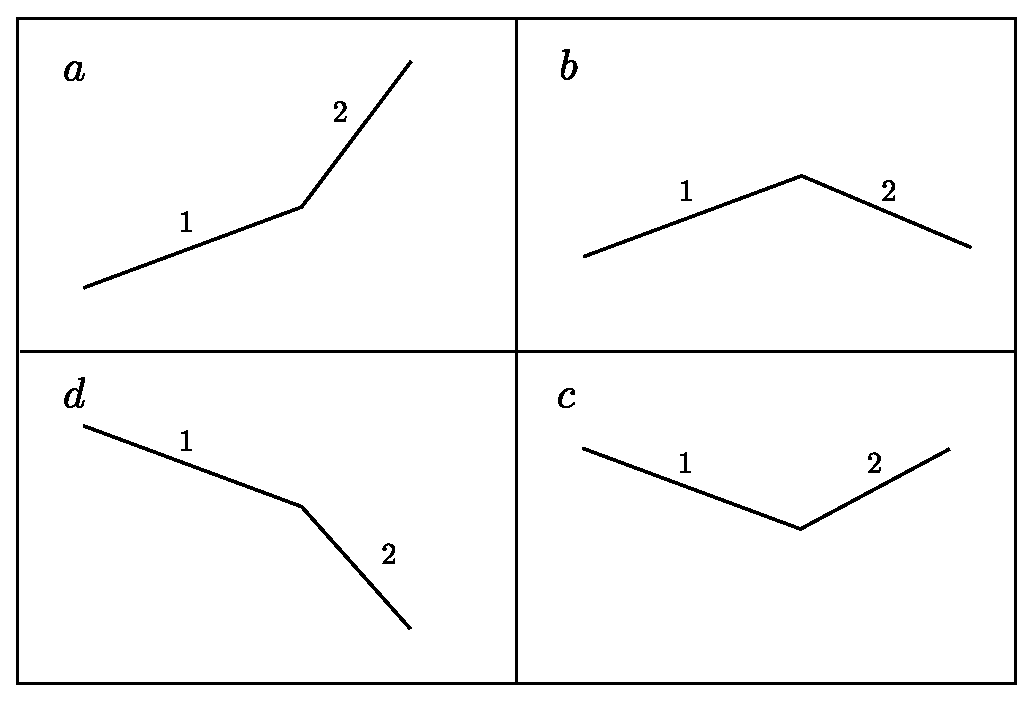
\includegraphics[width=\textwidth]{Rysunek0_all2.eps}
 \caption{Symbolic quadrant of response (second line) for market movement (first line)}
\end{figure}
\FloatBarrier

\begin{figure}[h]
\centering
\centering 
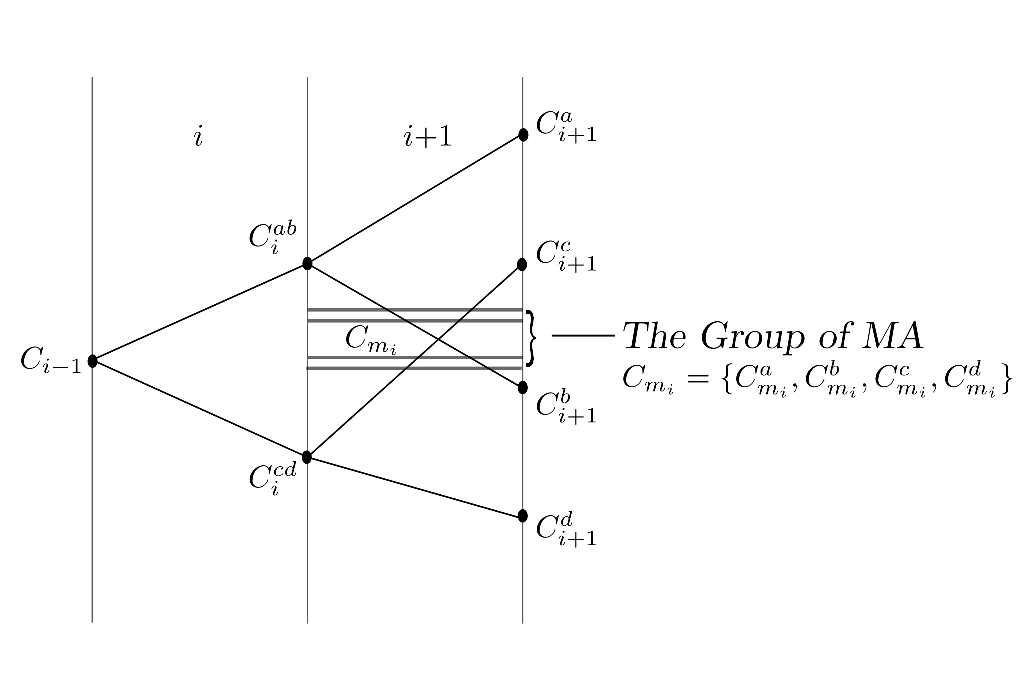
\includegraphics[width=\textwidth]{rysunek1pp.eps}
\caption{All versions}
\end{figure}
\FloatBarrier

\begin{figure}[h]
\centering
\begin{minipage}{.49\linewidth}
\centering 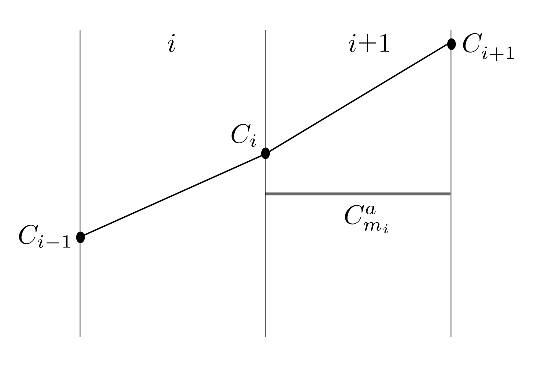
\includegraphics[width=\textwidth]{rysunek2a.eps}
\subcaption{Version a}
\label{jedno}
\end{minipage}
\begin{minipage}{.49\linewidth}
\centering 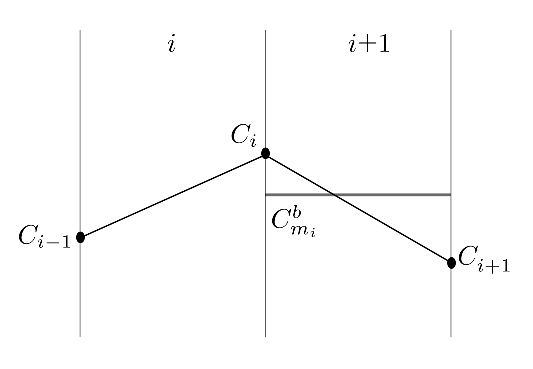
\includegraphics[width=\textwidth]{rysunek2b.eps}
\subcaption{Version b}
\label{dwu}
\end{minipage}
\\
\begin{minipage}{.49\linewidth}
\centering 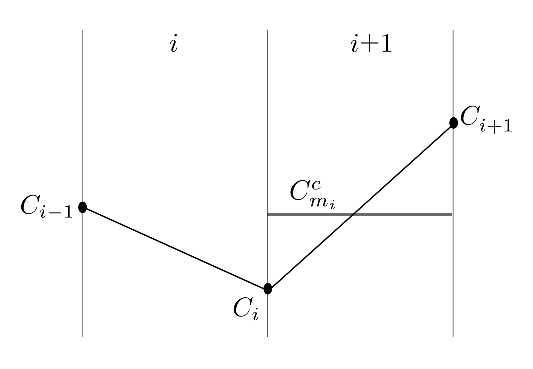
\includegraphics[width=\textwidth]{rysunek2c.eps}
\subcaption{Version c}
\label{cztero}
\end{minipage}
\begin{minipage}{.49\linewidth}
\centering 
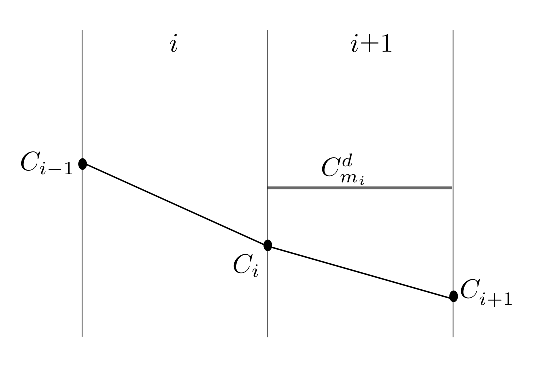
\includegraphics[width=\textwidth]{rysunek2d.eps}
\subcaption{Version d}
\label{mansard}
\end{minipage}
\caption{Separate strategies}
\end{figure}
\FloatBarrier


\section{The test results}
The study of strategy was carried out on the following markets:
currency pairs: EURUSD...
stock indexes: 
commodities: 

\begin{table}[!t]
\caption{Profits for all strategy quadrants} 
 \begin{center} 
 \begin{tabular}{|l|l|l|l|l|} 
 \hline \textbf{strategy} & \textbf{profit} & \textbf{bestCalmar} & \textbf{bestMALength} & \textbf{la} \\ \hline  
S1a & 26.177 & 5.5909868 & 24 & 2764\\ \hline 
S1b & -19.002 & -0.74976326 & 31 & 2801\\ \hline 
S1c & 12.025 & 2.6645247 & 31 & 2167\\ \hline 
S1d & -4.57 & -0.47001954 & 21 & 2226\\ \hline 
S1s & 14.33 & 2.957078 & NaN & 4968\\ 
\hline \end{tabular} 
 \end{center} 
 \end{table}
\FloatBarrier

\begin{figure}[h]
\centering
\begin{minipage}{.49\linewidth}
\centering 
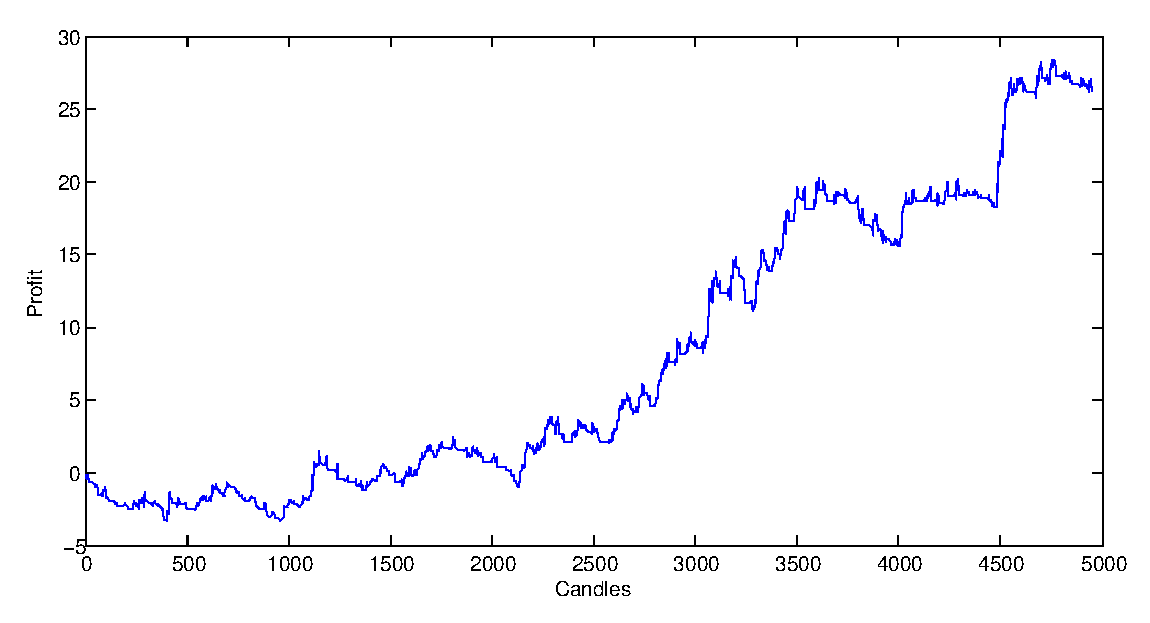
\includegraphics[width=0.82\textwidth]{S1a.eps}
\subcaption{Profit - S1a}
\label{jedno}
\end{minipage}
\begin{minipage}{.49\linewidth}
\centering 
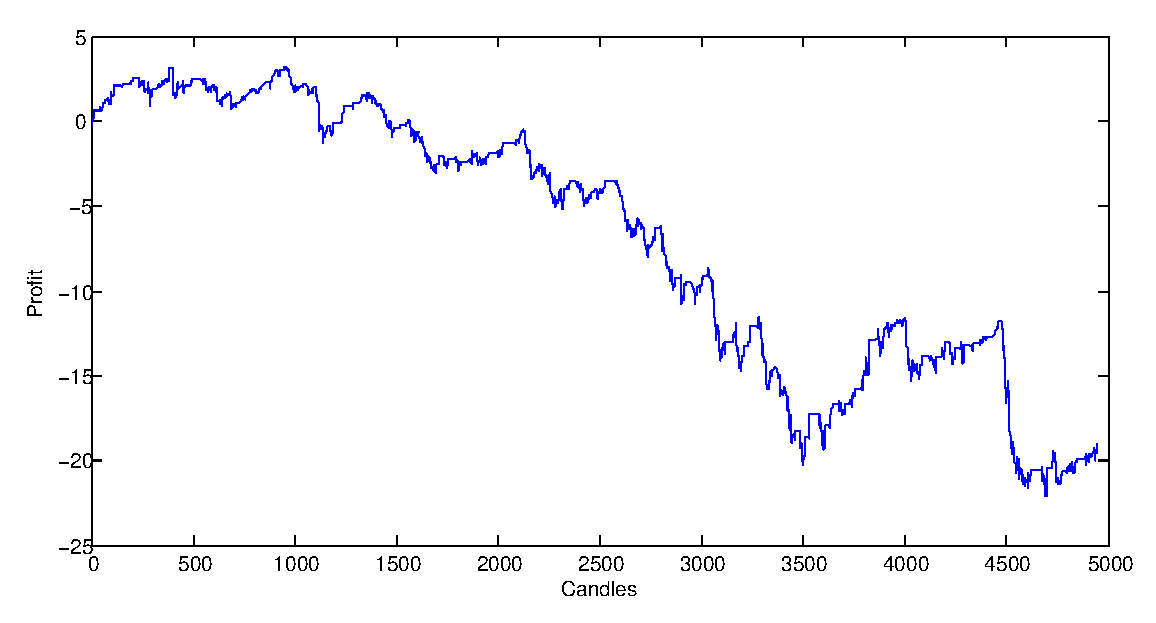
\includegraphics[width=0.82\textwidth]{S1b.eps}
\subcaption{Profit - S1b}
\label{dwu}
\end{minipage}
\\
\begin{minipage}{.49\linewidth}
\centering 
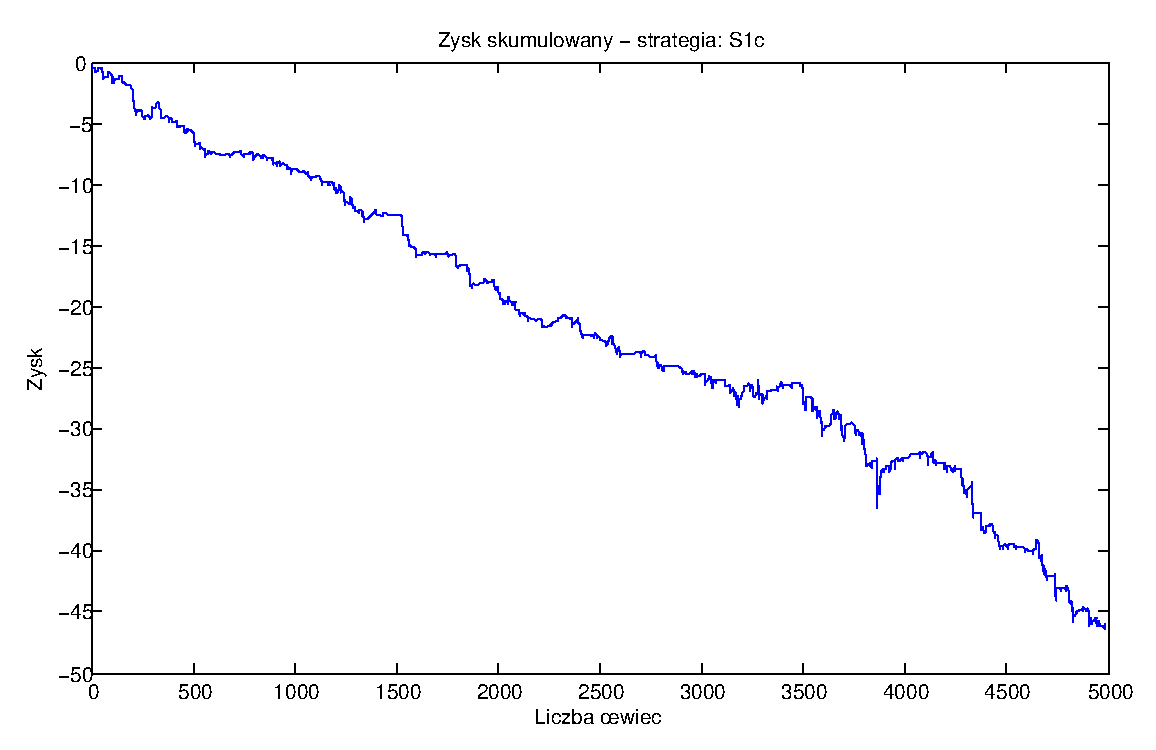
\includegraphics[width=0.82\textwidth]{S1c.eps}
\subcaption{Profit- S1c}
\label{cztero}
\end{minipage}
\begin{minipage}{.49\linewidth}
\centering 
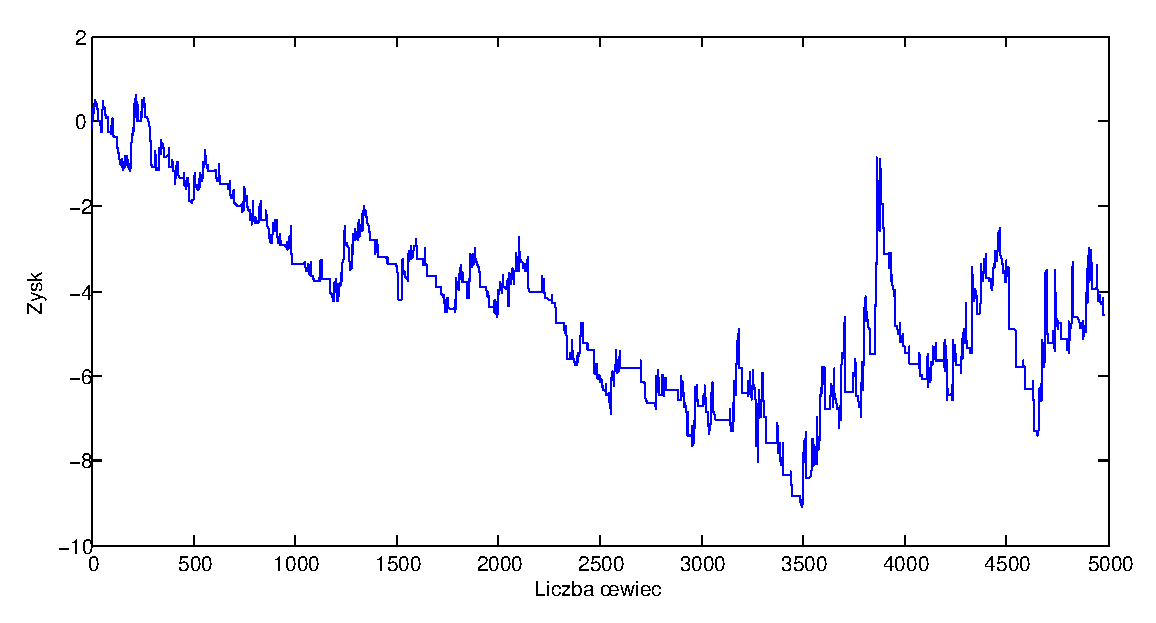
\includegraphics[width=0.82\textwidth]{S1d.eps}
\subcaption{Profit - S1d}
\label{mansard}
\end{minipage}
\begin{minipage}{\linewidth}
\centering 
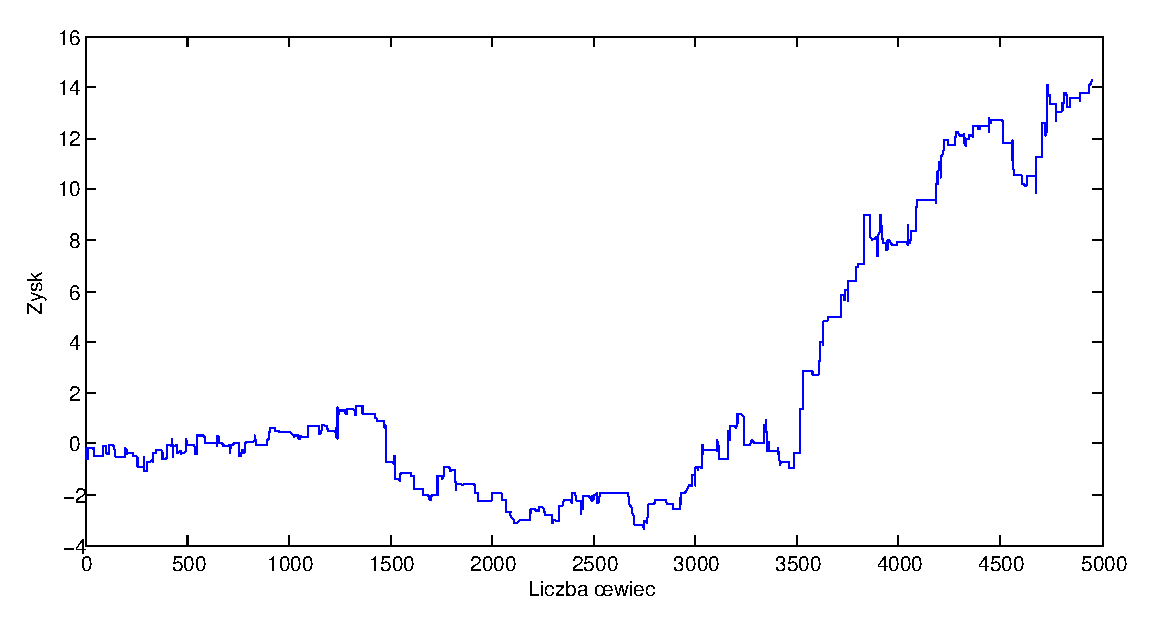
\includegraphics[width=0.6\textwidth]{S1s.eps}
\label{mansard}
\subcaption{Profit - S1s}
\end{minipage}
\caption{EURJPY market results}
\end{figure}
\FloatBarrier

\section{Conclusions}
\indent Suggested simple strategy is suitable only for algorithmic trading, even in absolute simplest form it seems to be interesting. As it’s been written in the introduction, more from cognitive point of view, than for the transaction value.\\
\indent This strategy can be modified in many ways.  Eg. in case of suggestions of simultaneous opening long and short positions better is to abandon work than opening both positions (due to transaction costs). The opening of another position in the same direction, eg. long position after closing the previous long position is senseless, it’s better to continue already opened position. These are two simplest ways to improve strategy. There are probably many ways to filter openings that allow to preserve only the most valuable due to profit events. Purpose of this paper was to prove the thesis, that even the simplest strategy has some potential profit, whose using is fascinating challenge.\\
\indent The authors believe, due to observing results of experiments, that the thesis of this dormant potential has been acknowledged. 



%%%%%%%%%% USE ____BIBTEX____ TO GENERATE YOUR REFERENCES 
%%%%%%%%%%% PLEASE UNCOMMENT THE TWO FOLLOWING LINES 

\bibliography{references-tewi}
\bibliographystyle{aiaa-tewi}



\end{document}